\begin{section}{MT}{Analyzing the CGM in the Massive Dark Matter Halos of \\
    \hspace*{4cm} Cosmological Simulations}{(Marius Tresoldi, Master Student)}
  \begin{minipage}{0.52\linewidth}
{\small In order to better understand the high redshift giant
      Ly-$\alpha$ nebulae revealed by MUSE, we analyze the properties of the
      hydrogen gas in the most massive dark matter halos at $z \sim 3$ using
      hydrodynamical simulations of cosmic structure formation such as the EAGLE
      and the Illustris project. These large-scale simulations have boxsizes of
      up to 100 cMpc and thus provide a useful sample of the rare halos of
      interest with $M >10^12.5 M_{\odot}$. Shown are both the phase diagram and
      the radial
      temperature distribution of the hydrogen gas in the RefL0100N1504
      simulation of EAGLE at $z=3.01$, where one can clearly distinguish between
      two phases. First there is the hot gas at $T \sim 10^{6.5} \mathrm{T}$ which
      corresponds to gas accreted from the intergalactic medium (IGM) that has
      been shock heated while falling into the gravitational potential well of
      the dark matter halo. The second phase is the cold CGM gas at $T \sim
      10^4.1 \mathrm{T}$ which is assumed to be responsible for the Ly-$\alpha$
      emission observed by MUSE when ionized by a central quasar.}
  \end{minipage}
  \hfill
  \begin{minipage}{0.42\linewidth}
      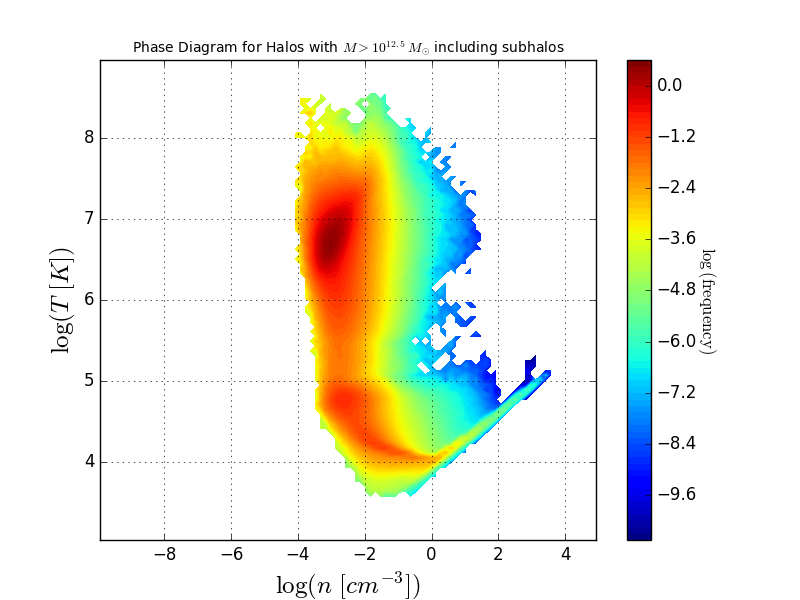
\includegraphics[height=12cm]{MT/PhaseDiagram.png}
      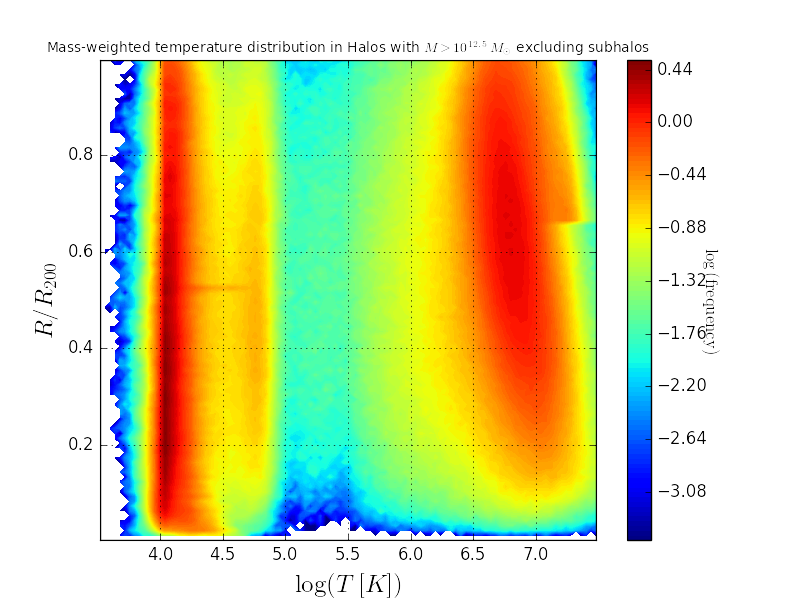
\includegraphics[height=12cm]{MT/T_R_dist.png}
  \end{minipage}
\end{section}
